\documentclass[12pt]{article}
\usepackage[utf8]{inputenc}
\usepackage[spanish]{babel}
\usepackage{graphicx}
\usepackage{float}
\title{Práctica 1\\Programación Evolutiva}
\author{Rafael Fernández López\\Ángel Valero Picazo}
\date{}

\pdfinfo
{
  /Title       (PRACTICA1-PE)
  /Author      (RAFAEL FERNANDEZ LOPEZ, ANGEL VALERO PICAZO)
}

\begin{document}

\maketitle
\newpage
\newpage
\tableofcontents
\newpage

\section{Estudio Obligatorio de las Funciones}	
	Para el estudio de las 5 funciones de la práctica se han fijado los siguientes valores:
	\begin{itemize}
		\item Tamaño de población : 100
		\item Número Máximo de Generaciones : 100
		\item Probabilidad de Cruce : 0.6
		\item Probabilidad de Mutación : 0.1
		\item Precisión : 0.0000001
	\end{itemize}

\subsection{Función 1}
	La primera función presenta un máximo de 1.98442121 en 0.98449933 como se puede observar en la figura.
\begin{figure}[H]
\centering
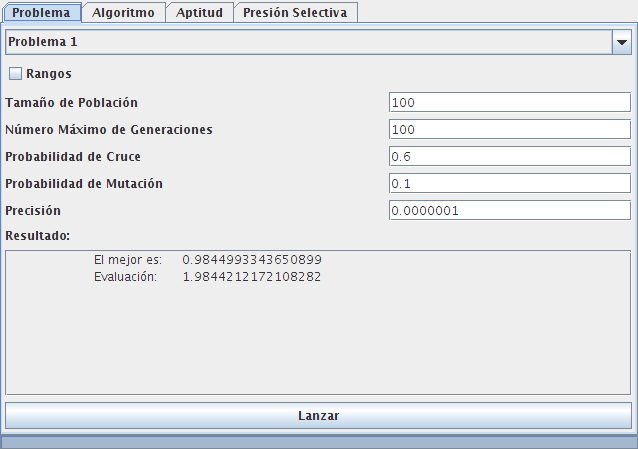
\includegraphics[scale=0.5]{graficas/F1inicial}
\caption{Función 1.}
\label{fig}
\end{figure}
	A continuación se muestran las diferentes gráficas para observar la evolución que sufre la función.

\subsubsection*{Gráfica Evaluación}
\begin{figure}[H]
\centering
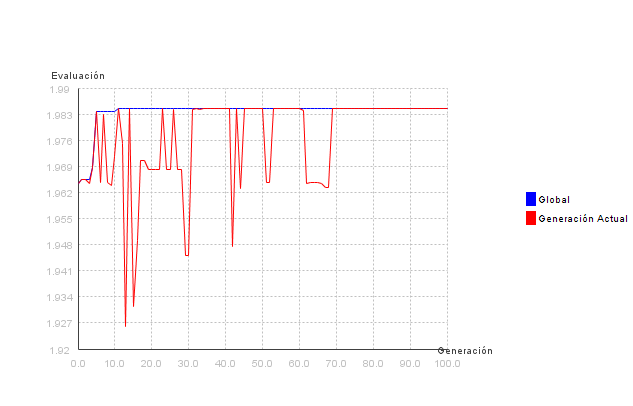
\includegraphics[scale=0.5]{graficas/F1inicial_algoritmo}
\caption{Gráfica evaluación.}
\label{fig}
\end{figure}

\subsubsection*{Gráfica Aptitud}
\begin{figure}[H]
\centering
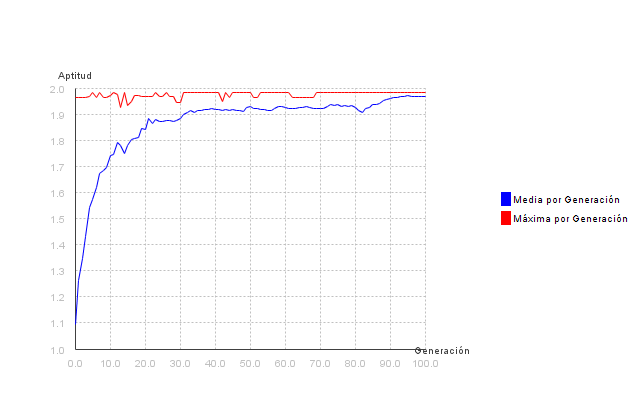
\includegraphics[scale=0.5]{graficas/F1inicial_aptitud}
\caption{Gráfica aptitud.}
\label{fig}
\end{figure}

\subsubsection*{Gráfica Presión Selectiva}
\begin{figure}[H]
\centering
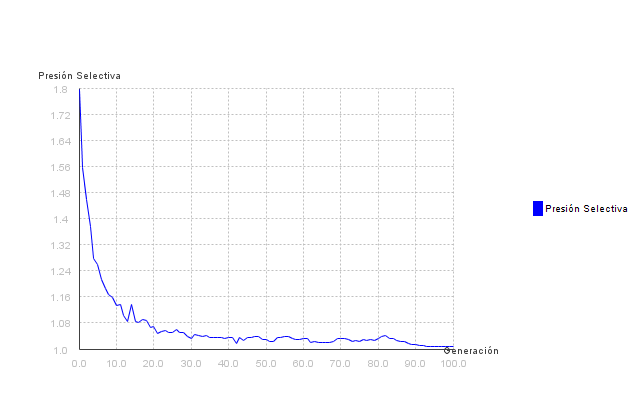
\includegraphics[scale=0.5]{graficas/F1inicial_presion}
\caption{Gráfica presión selectiva.}
\label{fig}
\end{figure}
\newpage

\subsection{Función 2}
	La segunda función presenta un máximo de 38.330 en 11.607 y 5.526 como se puede observar en la figura.
\begin{figure}[H]
\centering
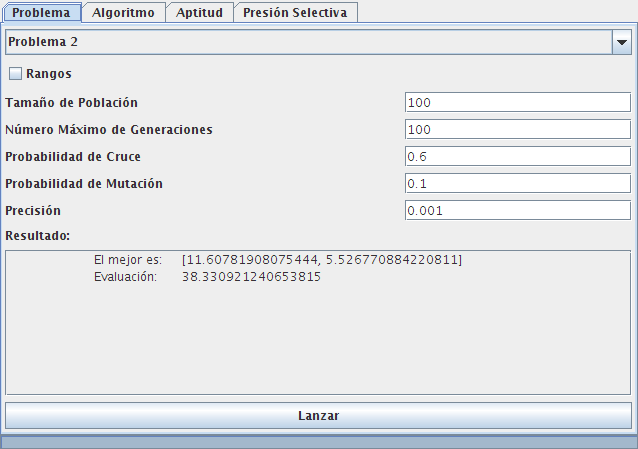
\includegraphics[scale=0.5]{graficas/F2inicial}
\caption{Función 2.}
\label{fig}
\end{figure}
	A continuación se muestran las diferentes gráficas para observar la evolución que sufre la función.

\subsubsection*{Gráfica Evaluación}
\begin{figure}[H]
\centering
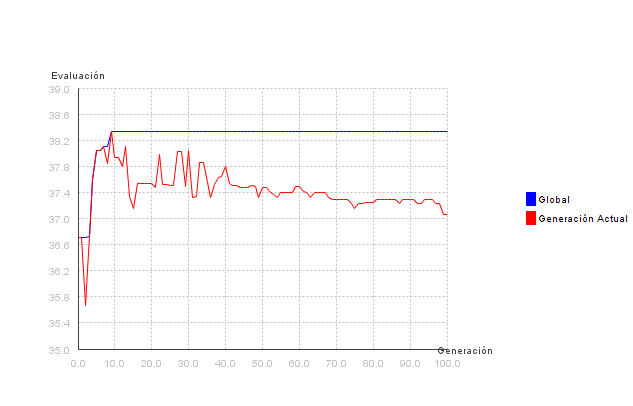
\includegraphics[scale=0.5]{graficas/F2inicial_algoritmo}
\caption{Gráfica evaluación.}
\label{fig}
\end{figure}

\subsubsection*{Gráfica Aptitud}
\begin{figure}[H]
\centering
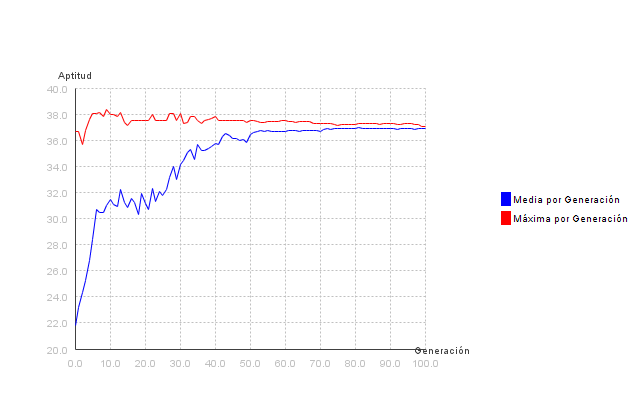
\includegraphics[scale=0.5]{graficas/F2inicial_aptitud}
\caption{Gráfica aptitud}
\label{fig}
\end{figure}

\subsubsection*{Gráfica Presión Selectiva}
\begin{figure}[H]
\centering
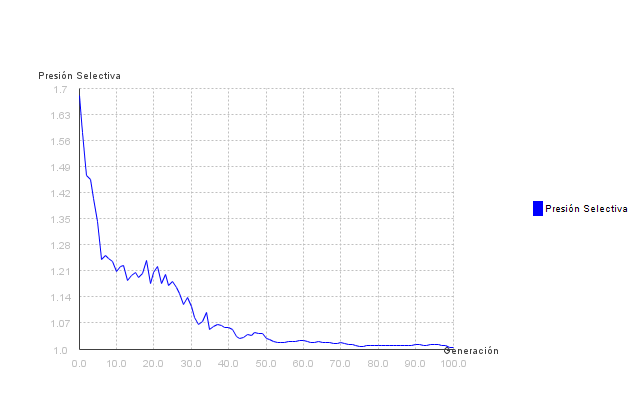
\includegraphics[scale=0.5]{graficas/F2inicial_presion}
\caption{Gráfica presión selectiva}
\label{fig}
\end{figure}
\newpage

\subsection{Función 3}
	La tercera función presenta un mínimo de -0.318067 en 4.574724 como se puede observar en la figura.
\begin{figure}[H]
\centering
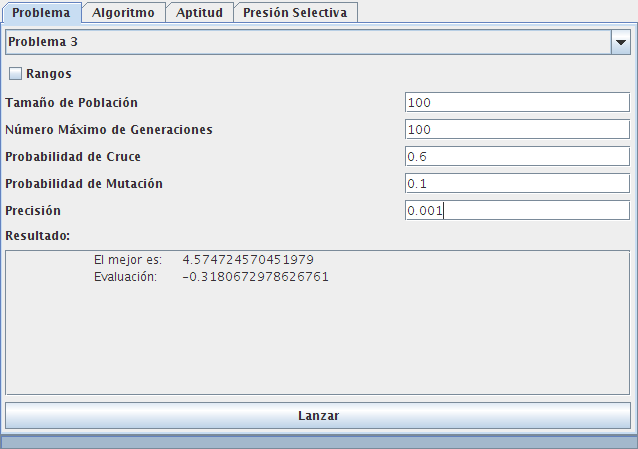
\includegraphics[scale=0.5]{graficas/F3inicial}
\caption{Función 3.}
\label{fig}
\end{figure}
	A continuación se muestran las diferentes gráficas para observar la evolución que sufre la función.

\subsubsection*{Gráfica Evaluación}
\begin{figure}[H]
\centering
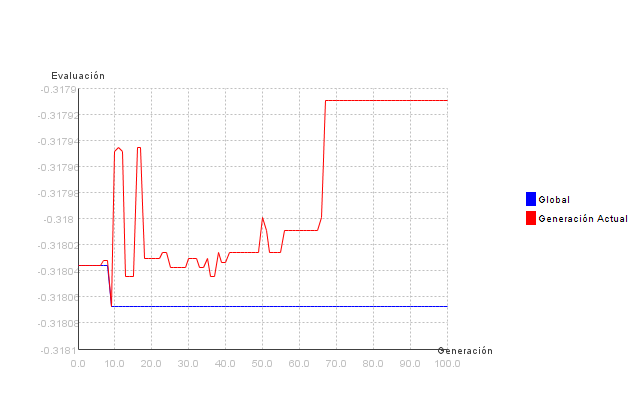
\includegraphics[scale=0.5]{graficas/F3inicial_algoritmo}
\caption{Gráfica evaluación.}
\label{fig}
\end{figure}

\subsubsection*{Gráfica Aptitud}
\begin{figure}[H]
\centering
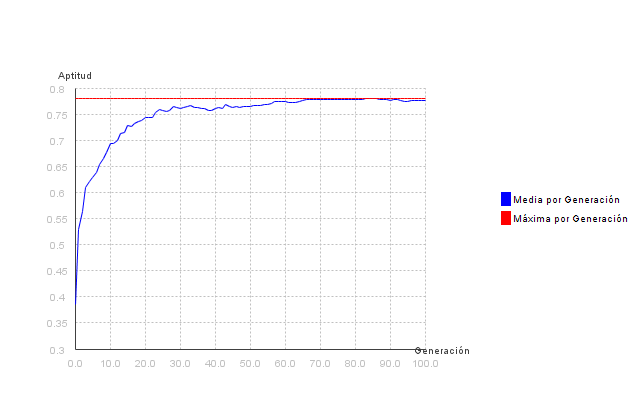
\includegraphics[scale=0.5]{graficas/F3inicial_aptitud}
\caption{Gráfica aptitud}
\label{fig}
\end{figure}

\subsubsection*{Gráfica Presión Selectiva}
\begin{figure}[H]
\centering
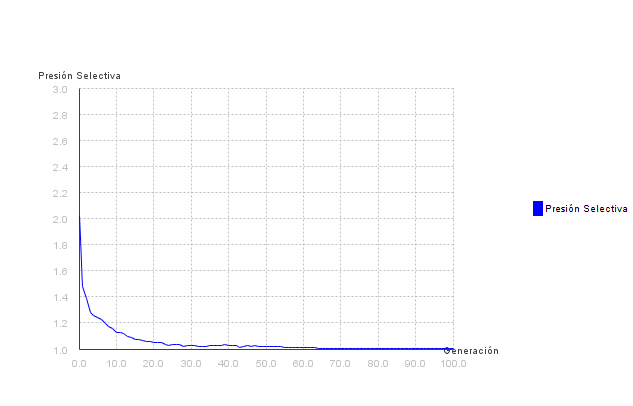
\includegraphics[scale=0.5]{graficas/F3inicial_presion}
\caption{Gráfica presión selectiva}
\label{fig}
\end{figure}
\newpage

\subsection{Función 4}
	La cuarta función presenta mínimos de -184.8932 en -0.7714 y -7.71 como se puede observar en la figura.
\begin{figure}[H]
\centering
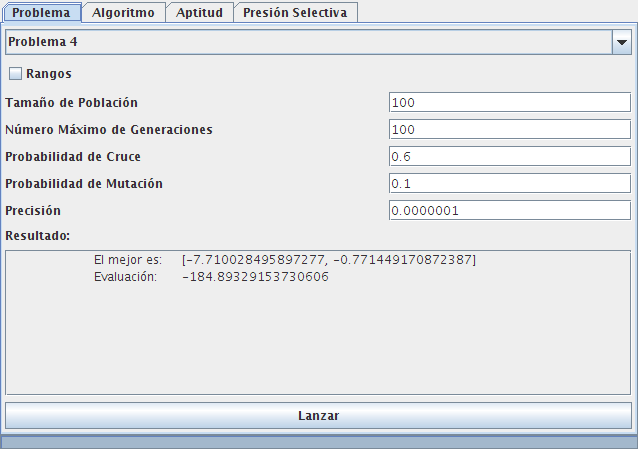
\includegraphics[scale=0.5]{graficas/F4inicial}
\caption{Función 4.}
\label{fig}
\end{figure}
	A continuación se muestran las diferentes gráficas para observar la evolución que sufre la función.

\subsubsection*{Gráfica Evaluación}
\begin{figure}[H]
\centering
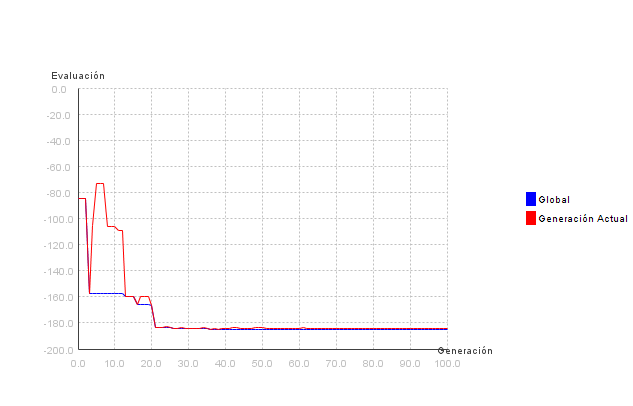
\includegraphics[scale=0.5]{graficas/F4inicial_algoritmo}
\caption{Gráfica evaluación.}
\label{fig}
\end{figure}

\subsubsection*{Gráfica Aptitud}
\begin{figure}[H]
\centering
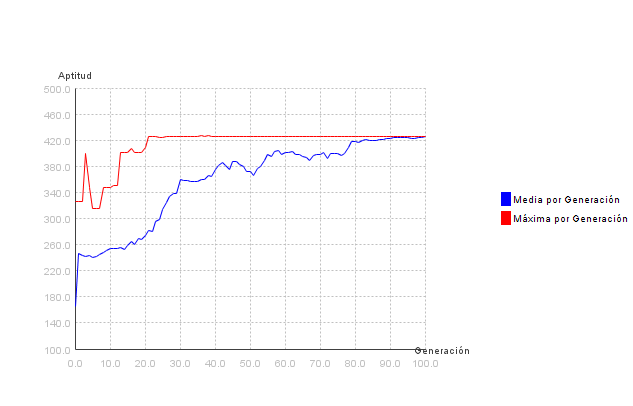
\includegraphics[scale=0.5]{graficas/F4inicial_aptitud}
\caption{Gráfica aptitud}
\label{fig}
\end{figure}

\subsubsection*{Gráfica Presión Selectiva}
\begin{figure}[H]
\centering
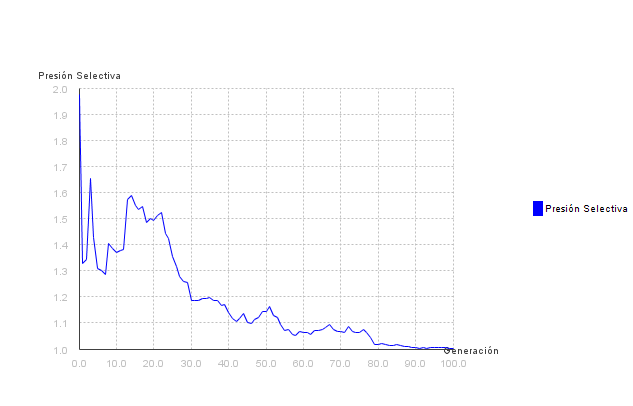
\includegraphics[scale=0.5]{graficas/F4inicial_presion}
\caption{Gráfica presión selectiva}
\label{fig}
\end{figure}
\newpage

\subsection{Función 5}
	La quinta función presenta un mínimos de -3.635715 cuando n=4 como se puede observar en la figura.
\begin{figure}[H]
\centering
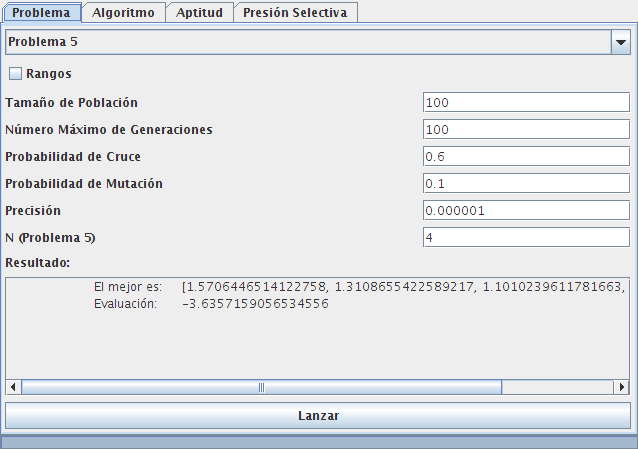
\includegraphics[scale=0.5]{graficas/F5inicial}
\caption{Función 5.}
\label{fig}
\end{figure}
	A continuación se muestran las diferentes gráficas para observar la evolución que sufre la función.

\subsubsection*{Gráfica Evaluación}
\begin{figure}[H]
\centering
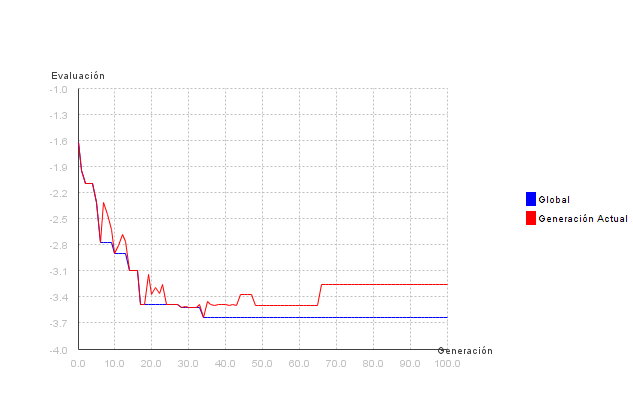
\includegraphics[scale=0.5]{graficas/F5inicial_algoritmo}
\caption{Gráfica evaluación.}
\label{fig}
\end{figure}

\subsubsection*{Gráfica Aptitud}
\begin{figure}[H]
\centering
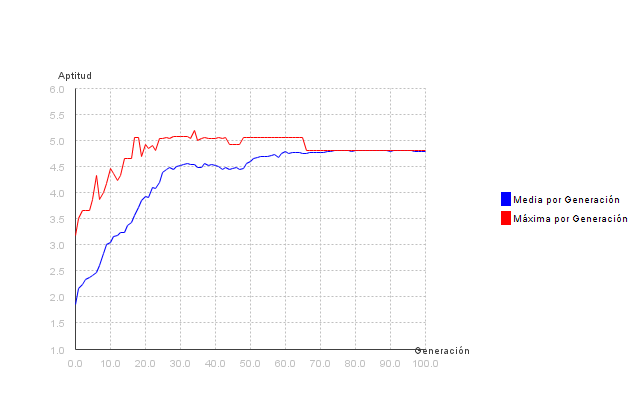
\includegraphics[scale=0.5]{graficas/F5inicial_aptitud}
\caption{Gráfica aptitud}
\label{fig}
\end{figure}

\subsubsection*{Gráfica Presión Selectiva}
\begin{figure}[H]
\centering
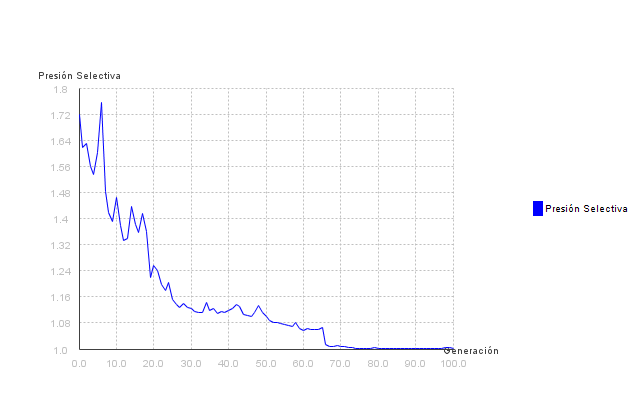
\includegraphics[scale=0.5]{graficas/F5inicial_presion}
\caption{Gráfica presión selectiva}
\label{fig}
\end{figure}
\newpage

\section{Estudio Opcional de las Funciones}	
	Para el estudio de las 5 funciones de la práctica se han fijado los siguientes valores:
	\begin{itemize}
		\item Tamaño de población : 100
		\item Número Máximo de Generaciones : 100
		\item Probabilidad de Cruce : 0.6
		\item Probabilidad de Mutación : 0.1
		\item Precisión : 0.0000001
	\end{itemize}
	A la hora de estudiar la influencia de un cierto parámetro hay que indicar el rango de valores y el incremento de cada iteración. Los demás parámetros se quedan fijados con los valores anteriores.
\subsection{Función 1}
\subsubsection*{Estudio Tamaño de Población}
	Se varia el tamaño de la población de 10 a 460 en incrementos de 50.
%tabla
\begin{table}[H]
\begin{center}
\begin{tabular}{|cc|} \hline
Tamaño Población & Máximo Obtenido \\  \hline
10  & 1.95300216 \\ 
60  & 1.97934328 \\ 
110 & 1.98414916 \\
160 & 1.98371034 \\
210 & 1.98417869 \\
260 & 1.98442445 \\
310 & 1.98441514 \\
360 & 1.98442447 \\ 
410 & 1.98441983 \\
460 & 1.98442446 \\  \hline
\end{tabular}
\end{center}
\end{table}
 

\subsubsection*{Estudio Número Máximo de Generaciones}
	Se varia el número máximo de generaciones de 10 a 460 en incrementos de 50.
%tabla
\begin{table}[H]
\begin{center}
\begin{tabular}{|cc|} \hline
Número Máximo Generaciones & Máximo Obtenido \\  \hline
10  & 1.98420692 \\ 
60  & 1.98371961 \\ 
110 & 1.98428048 \\
160 & 1.98440826 \\
210 & 1.98428711 \\
260 & 1.98312992 \\
310 & 1.98398901 \\
360 & 1.98415210 \\ 
410 & 1.98441996 \\
460 & 1.98437203 \\  \hline
\end{tabular}
\end{center}
\end{table}
\subsubsection*{Estudio Probabilidad de Cruce}
	Se varia la probabilidad de cruce de 0.1 a 1 en incrementos de 0.1.
%tabla
\begin{table}[H]
\begin{center}
\begin{tabular}{|cc|} \hline
Probabilidad Cruce & Máximo Obtenido \\  \hline
0.1 & 1.96842359 \\ 
0.2 & 1.98435401 \\ 
0.3 & 1.98146319 \\
0.4 & 1.95309093 \\
0.5 & 1.98430322 \\
0.6 & 1.95271094 \\
0.7 & 1.98437476 \\
0.8 & 1.98441772 \\ 
0.9 & 1.98364390 \\
1   & 1.98392662 \\  \hline
\end{tabular}
\end{center}
\end{table}
\subsubsection*{Estudio Probabilidad de Mutación}
	Se varia la probabilidad de mutación de 0.1 a 1 en incrementos de 0.1.
%tabla
\begin{table}[H]
\begin{center}
\begin{tabular}{|cc|} \hline
Probabilidad Mutación & Máximo Obtenido \\  \hline
0.1 & 1.98437036 \\ 
0.2 & 1.98427642 \\ 
0.3 & 1.98003732 \\
0.4 & 1.95247656 \\
0.5 & 1.98440824 \\
0.6 & 1.98440908 \\
0.7 & 1.98437398 \\
0.8 & 1.98434554 \\ 
0.9 & 1.98274766 \\
1   & 1.98261901 \\  \hline
\end{tabular}
\end{center}
\end{table}
\subsubsection*{Estudio Precisión}
	Se varia la precisión de 0.00000001 a 0.0000001 en incrementos de 0.00000001.
%tabla
\begin{table}[H]
\begin{center}
\begin{tabular}{|cc|} \hline
Precisión & Máximo Obtenido \\  \hline
0.00000001 & 1.98439835 \\ 
0.00000002 & 1.98436467 \\ 
0.00000003 & 1.98381407 \\
0.00000004 & 1.98425537 \\
0.00000005 & 1.98424478 \\
0.00000006 & 1.98437295 \\
0.00000007 & 1.98398618 \\
0.00000008 & 1.98441399 \\ 
0.00000009 & 1.98442388 \\
0.00000010 & 1.98442446 \\  \hline
\end{tabular}
\end{center}
\end{table}

\subsection{Función 2}
\subsubsection*{Estudio Tamaño de Población}
	Se varia el tamaño de la población de 10 a 460 en incrementos de 50.
%tabla
\begin{table}[H]
\begin{center}
\begin{tabular}{|cc|} \hline
Tamaño Población & Máximo Obtenido \\  \hline
10  & 27.814 \\ 
60  & 36.559 \\ 
110 & 36.542 \\
160 & 38.349 \\
210 & 37.983 \\
260 & 38.198 \\
310 & 38.709 \\
360 & 38.444 \\ 
410 & 38.557 \\
460 & 38.825 \\  \hline
\end{tabular}
\end{center}
\end{table}
 

\subsubsection*{Estudio Número Máximo de Generaciones}
	Se varia el número máximo de generaciones de 10 a 460 en incrementos de 50.
%tabla
\begin{table}[H]
\begin{center}
\begin{tabular}{|cc|} \hline
Número Máximo Generaciones & Máximo Obtenido \\  \hline
10  & 36.809 \\ 
60  & 38.107 \\ 
110 & 37.408 \\
160 & 37.132 \\
210 & 38.525 \\
260 & 37.483 \\
310 & 37.196 \\
360 & 38.595 \\ 
410 & 37.645 \\
460 & 37.806 \\  \hline
\end{tabular}
\end{center}
\end{table}
\subsubsection*{Estudio Probabilidad de Cruce}
	Se varia la probabilidad de cruce de 0.1 a 1 en incrementos de 0.1.
%tabla
\begin{table}[H]
\begin{center}
\begin{tabular}{|cc|} \hline
Probabilidad Cruce & Máximo Obtenido \\  \hline
0.1 & 37.629 \\ 
0.2 & 38.146 \\ 
0.3 & 36.738 \\
0.4 & 37.894 \\
0.5 & 38.746 \\
0.6 & 37.302 \\
0.7 & 36.948 \\
0.8 & 38.793 \\ 
0.9 & 37.733 \\
1   & 38.683 \\  \hline
\end{tabular}
\end{center}
\end{table}
\subsubsection*{Estudio Probabilidad de Mutación}
	Se varia la probabilidad de mutación de 0.1 a 1 en incrementos de 0.1.
%tabla
\begin{table}[H]
\begin{center}
\begin{tabular}{|cc|} \hline
Probabilidad Mutación & Máximo Obtenido \\  \hline
0.1 & 38.091 \\ 
0.2 & 38.719 \\ 
0.3 & 38.039 \\
0.4 & 37.945 \\
0.5 & 38.532 \\
0.6 & 38.450 \\
0.7 & 37.630 \\
0.8 & 37.748 \\ 
0.9 & 38.091 \\
1   & 36.527 \\  \hline
\end{tabular}
\end{center}
\end{table}
\subsubsection*{Estudio Precisión}
	Se varia la precisión de 0.00000001 a 0.0000001 en incrementos de 0.00000001.
%tabla
\begin{table}[H]
\begin{center}
\begin{tabular}{|cc|} \hline
Precisión & Máximo Obtenido \\  \hline
0.00000001 & 36.722 \\ 
0.00000002 & 38.447 \\ 
0.00000003 & 35.648 \\
0.00000004 & 37.240 \\
0.00000005 & 38.647 \\
0.00000006 & 38.323 \\
0.00000007 & 38.451\\
0.00000008 & 37.847 \\ 
0.00000009 & 37.600 \\
0.00000010 & 37.837 \\  \hline
\end{tabular}
\end{center}
\end{table}

\subsection{Función 3}
\subsubsection*{Estudio Tamaño de Población}
	Se varia el tamaño de la población de 10 a 460 en incrementos de 50.
%tabla
\begin{table}[H]
\begin{center}
\begin{tabular}{|cc|} \hline
Tamaño Población & Mínimo Obtenido \\  \hline
10  & -0.269028 \\ 
60  & -0.317650 \\ 
110 & -0.316676 \\
160 & -0.318071 \\
210 & -0.318069 \\
260 & -0.318071 \\
310 & -0.318071 \\
360 & -0.318071 \\ 
410 & -0.318071 \\
460 & -0.318071 \\  \hline
\end{tabular}
\end{center}
\end{table}
 

\subsubsection*{Estudio Número Máximo de Generaciones}
	Se varia el número máximo de generaciones de 10 a 460 en incrementos de 50.
%tabla
\begin{table}[H]
\begin{center}
\begin{tabular}{|cc|} \hline
Número Máximo Generaciones & Mínimo Obtenido \\  \hline
10  & -0.318035 \\ 
60  & -0.318071 \\ 
110 & -0.318071 \\
160 & -0.318061 \\
210 & -0.318071 \\
260 & -0.316046 \\
310 & -0.316980 \\
360 & -0.318070 \\ 
410 & -0.318071 \\
460 & -0.318038 \\  \hline
\end{tabular}
\end{center}
\end{table}
\subsubsection*{Estudio Probabilidad de Cruce}
	Se varia la probabilidad de cruce de 0.1 a 1 en incrementos de 0.1.
%tabla
\begin{table}[H]
\begin{center}
\begin{tabular}{|cc|} \hline
Probabilidad Cruce & Mínimo Obtenido \\  \hline
0.1 & -0.317957 \\ 
0.2 & -0.315544 \\ 
0.3 & -0.318038 \\
0.4 & -0.317997 \\
0.5 & -0.318056 \\
0.6 & -0.318048 \\
0.7 & -0.318071 \\
0.8 & -0.318071 \\ 
0.9 & -0.318069 \\
1   & -0.315809 \\  \hline
\end{tabular}
\end{center}
\end{table}
\subsubsection*{Estudio Probabilidad de Mutación}
	Se varia la probabilidad de mutación de 0.1 a 1 en incrementos de 0.1.
%tabla
\begin{table}[H]
\begin{center}
\begin{tabular}{|cc|} \hline
Probabilidad Mutación & Mínimo Obtenido \\  \hline
0.1 & -0.318067 \\ 
0.2 & -0.317451 \\ 
0.3 & -0.318071 \\
0.4 & -0.318070 \\
0.5 & -0.318051 \\
0.6 & -0.318068 \\
0.7 & -0.318054 \\
0.8 & -0.318071 \\ 
0.9 & -0.318031 \\
1   & -0.318071 \\  \hline
\end{tabular}
\end{center}
\end{table}
\subsubsection*{Estudio Precisión}
	Se varia la precisión de 0.00000001 a 0.0000001 en incrementos de 0.00000001.
%tabla
\begin{table}[H]
\begin{center}
\begin{tabular}{|cc|} \hline
Precisión & Mínimo Obtenido \\  \hline
0.00000001 & -0.318061 \\ 
0.00000002 & -0.318043 \\ 
0.00000003 & -0.318070 \\
0.00000004 & -0.318069 \\
0.00000005 & -0.317839 \\
0.00000006 & -0.316134 \\
0.00000007 & -0.317775 \\
0.00000008 & -0.317918 \\ 
0.00000009 & -0.318071 \\
0.00000010 & -0.318071 \\  \hline
\end{tabular}
\end{center}
\end{table}

\subsection{Función 4}
\subsubsection*{Estudio Tamaño de Población}
	Se varia el tamaño de la población de 10 a 460 en incrementos de 50.
%tabla
\begin{table}[H]
\begin{center}
\begin{tabular}{|cc|} \hline
Tamaño Población & Mínimo Obtenido \\  \hline
10  & -72.9491 \\ 
60  & -111.6176 \\ 
110 & -135.3392 \\
160 & -164.1953 \\
210 & -186.7028 \\
260 & -122.3201 \\
310 & -186.6605 \\
360 & -186.4939 \\ 
410 & -186.6807 \\
460 & -183.2034 \\  \hline
\end{tabular}
\end{center}
\end{table}
 

\subsubsection*{Estudio Número Máximo de Generaciones}
	Se varia el número máximo de generaciones de 10 a 460 en incrementos de 50.
%tabla
\begin{table}[H]
\begin{center}
\begin{tabular}{|cc|} \hline
Número Máximo Generaciones & Mínimo Obtenido \\  \hline
10  & -184.9346 \\ 
60  & -92.6084 \\ 
110 & -130.5393 \\
160 & -181.9670 \\
210 & -186.0169 \\
260 & -186.1944 \\
310 & -181.9110 \\
360 & -172.6664 \\ 
410 & -180.1084 \\
460 & -183.5149 \\  \hline
\end{tabular}
\end{center}
\end{table}
\subsubsection*{Estudio Probabilidad de Cruce}
	Se varia la probabilidad de cruce de 0.1 a 1 en incrementos de 0.1.
%tabla
\begin{table}[H]
\begin{center}
\begin{tabular}{|cc|} \hline
Probabilidad Cruce & Mínimo Obtenido \\  \hline
0.1 & -183.4316 \\ 
0.2 & -185.9303 \\ 
0.3 & -129.8455 \\
0.4 & -173.6409 \\
0.5 & -78.5388 \\
0.6 & -167.1205 \\
0.7 & -146.5928 \\
0.8 & -185.6488 \\ 
0.9 & -185.7041 \\
1   & -185.5169 \\  \hline
\end{tabular}
\end{center}
\end{table}
\subsubsection*{Estudio Probabilidad de Mutación}
	Se varia la probabilidad de mutación de 0.1 a 1 en incrementos de 0.1.
%tabla
\begin{table}[H]
\begin{center}
\begin{tabular}{|cc|} \hline
Probabilidad Mutación & Mínimo Obtenido \\  \hline
0.1 & -181.7142 \\ 
0.2 & -186.3339 \\ 
0.3 & -184.8755 \\
0.4 & -168.8033 \\
0.5 & -176.6376 \\
0.6 & -186.1045 \\
0.7 & -186.0351 \\
0.8 & -130.8406 \\ 
0.9 & -176.9818 \\
1   & -117.5346 \\  \hline
\end{tabular}
\end{center}
\end{table}
\subsubsection*{Estudio Precisión}
	Se varia la precisión de 0.00000001 a 0.0000001 en incrementos de 0.00000001.
%tabla
\begin{table}[H]
\begin{center}
\begin{tabular}{|cc|} \hline
Precisión & Mínimo Obtenido \\  \hline
0.00000001 & -157.2270 \\ 
0.00000002 & -100.5084 \\ 
0.00000003 & -182.6262 \\
0.00000004 & -182.6732 \\
0.00000005 & -175.5188 \\
0.00000006 & -156.3064 \\
0.00000007 & -186.4751 \\
0.00000008 & -183.7943 \\ 
0.00000009 & -182.0350 \\
0.00000010 & -103.3778 \\  \hline
\end{tabular}
\end{center}
\end{table}

\subsection{Función 5}
	Estudio realizado con el parámetro n=2
\subsubsection*{Estudio Tamaño de Población}
	Se varia el tamaño de la población de 10 a 460 en incrementos de 50.
%tabla
\begin{table}[H]
\begin{center}
\begin{tabular}{|cc|} \hline
Tamaño Población & Mínimo Obtenido \\  \hline
10  & -1.796137 \\ 
60  & -1.814462 \\ 
110 & -1.946951 \\
160 & -1.958608 \\
210 & -1.957552 \\
260 & -1.955446 \\
310 & -1.957697 \\
360 & -1.951744 \\ 
410 & -1.957041 \\
460 & -1.959072 \\  \hline
\end{tabular}
\end{center}
\end{table}
 

\subsubsection*{Estudio Número Máximo de Generaciones}
	Se varia el número máximo de generaciones de 10 a 460 en incrementos de 50.
%tabla
\begin{table}[H]
\begin{center}
\begin{tabular}{|cc|} \hline
Número Máximo Generaciones & Mínimo Obtenido \\  \hline
10  & -1.881701 \\ 
60  & -1.956846 \\ 
110 & -1.952919 \\
160 & -1.955062 \\
210 & -1.955691 \\
260 & -1.913593 \\
310 & -1.942198 \\
360 & -1.957594 \\ 
410 & -1.928775 \\
460 & -1.939548 \\  \hline
\end{tabular}
\end{center}
\end{table}
\subsubsection*{Estudio Probabilidad de Cruce}
	Se varia la probabilidad de cruce de 0.1 a 1 en incrementos de 0.1.
%tabla
\begin{table}[H]
\begin{center}
\begin{tabular}{|cc|} \hline
Probabilidad Cruce & Mínimo Obtenido \\  \hline
0.1 & -1.812777 \\ 
0.2 & -1.959031 \\ 
0.3 & -1.954478 \\
0.4 & -1.693149 \\
0.5 & -1.862722 \\
0.6 & -1.907169 \\
0.7 & -1.916014 \\
0.8 & -1.957601 \\ 
0.9 & -1.790226 \\
1   & -1.957731 \\  \hline
\end{tabular}
\end{center}
\end{table}
\subsubsection*{Estudio Probabilidad de Mutación}
	Se varia la probabilidad de mutación de 0.1 a 1 en incrementos de 0.1.
%tabla
\begin{table}[H]
\begin{center}
\begin{tabular}{|cc|} \hline
Probabilidad Mutación & Mínimo Obtenido \\  \hline
0.1 & -1.958825 \\ 
0.2 & -1.955002 \\ 
0.3 & -1.954345 \\
0.4 & -1.958458 \\
0.5 & -1.784000 \\
0.6 & -1.958566 \\
0.7 & -1.936031 \\
0.8 & -1.937824 \\ 
0.9 & -1.958157 \\
1   & -1.948154 \\  \hline
\end{tabular}
\end{center}
\end{table}
\subsubsection*{Estudio Precisión}
	Se varia la precisión de 0.00000001 a 0.0000001 en incrementos de 0.00000001.
%tabla
\begin{table}[H]
\begin{center}
\begin{tabular}{|cc|} \hline
Precisión & Mínimo Obtenido \\  \hline
0.00000001 & -1.954301 \\ 
0.00000002 & -1.952432 \\ 
0.00000003 & -1.956418 \\
0.00000004 & -1.953366 \\
0.00000005 & -1.918998 \\
0.00000006 & -1.956360 \\
0.00000007 & -1.935455 \\
0.00000008 & -1.900311 \\ 
0.00000009 & -1.917352 \\
0.00000010 & -1.946798 \\  \hline
\end{tabular}
\end{center}
\end{table}


\end{document}
